\section{Introduction} \label{section:introduction}
The remarkable rise in the capability of large language models (LLMs) gives hope that they could be used to provide many kinds of mental health talk therapy. Indeed, one can simply ask for such help from an online LLM and possibly receive good help \citep{Siddals2024}.  Since this is a medical intervention, it should be grounded in evidence that shows its effectiveness.

Our goal is to automate a specific type of talk therapy focusing on the problem of tobacco addiction with the specific goal of moving \emph{ambivalent smokers} towards the decision to quit. Ambivalent smokers know that smoking is bad for them but continue smoking because of its positive effects \emph{and} because they don't spend much time contemplating their smoking behaviour \citep{miller1983motivational,rollnick1997helping,MillerRollnick2023}.  More than 50\% of all smokers are in this ambivalent state \cite{Babb2017}, and so moving even a small fraction of these towards the decision to quit could have a major impact. The \emph{Motivational Interviewing} (MI) talk therapy approach \citep{MillerRollnick2023} is often employed by counsellors to guide smokers away from their ambivalent state towards the decision to quit. This decision is a key precursor for any successful attempt to quit \citep{West2006}.

There has been significant activity in recent years on automating talk therapy in many domains, including the use of MI to help in smoking cessation \citep{10.1145/3652988.3673932,basar-etal-2024-extent,welivita-pu-2023-boosting,info:doi/10.2196/49132}. \citet{info:doi/10.2196/49132}, the predecessor of the present work, developed \oldsysname which showed that a partially scripted and partially generative chatbot could significantly change smokers' readiness to quit. However, scripting with limited generation restricts the natural flow of conversation, thereby preventing full utilization  of MI elements. \citet{10.1145/3652988.3673932} show the effectiveness of a fully-generative chatbot focused on alcohol use. As well, more complete MI administered by human counsellors has shown a much greater impact \citep{Boudreaux2012}. This, together with the potential availability of always-accessible, lower-cost counselling, forms the motivation for this work.

In this paper, we describe the design and measurement of a single, large prompt of a state-of-the-art LLM-based chatbot called \textbf{\sysname} \footnote{This paper describes \sysnamewithv and compares it with our previous work, \oldsysname \citep{info:doi/10.2196/49132}. Our group's broader goal is to iteratively develop MI-based chatbots for smoking cessation. See Appendix~\ref{appendix:mibot_version_list} for a comprehensive list of all previous MI chatbot iterations. Unless otherwise noted, \sysname refers to \sysnamewithv.}. A key to our approach is that expert MI clinicians and researchers participated in designing the prompt and evaluating the chatbot. We iteratively evolved the prompt with the help of MI experts, LLM-simulated smokers, and humans role-playing as smokers.

\sysname was then tested on smokers recruited online (for pay) to measure both the effect on their confidence to quit and the quality of the conversations in four ways:\vspace{-0.2em}
\begin{enumerate}[itemsep=0pt, parsep=0pt]
    \item The participants' readiness to quit through a widely used \emph{readiness ruler} \citep{Boudreaux2012} before the conversation and one week later. The difference between these two measurements is our primary metric of effectiveness.
    \item A rating of the perceived empathy of the chatbot on the \textbf{CARE} scale \citep{10.1093/fampra/cmh621}, which is widely used to assess the quality of the clinician-patient interaction and clinician empathy.
    \item A measurement of how well the counsellor's utterances adhere to the standards of MI based on the Motivational Interviewing Skill Code (\textbf{MISC}) \citep{MISC}.
    \item The percentage of client utterances that reflect their motivation to change their smoking behaviour as a portion of the total number of utterances that reflect either change or the sustaining of their behaviour --- also based on MISC.
\end{enumerate}

The key contributions of this paper are:\vspace{-0.2em}
\begin{enumerate}[itemsep=0pt, parsep=0pt]
    \item An expert-informed chatbot that performs fully generative MI counselling.
    \item Measurements of effectiveness on human smokers.
    \item A validated automated system to measure the adherence of counsellor chatbot utterances to the precepts of MI.
    \item A validated automated measurement of the effect of the chatbot on the client's motivation through analysis of their language.
    \item A dataset of the transcripts of  $106$ chatbot-human conversations together with measured outcomes of effectiveness, perceived empathy, and utterance-level MISC annotations \footnote{\texttt{\href{https://github.com/cimhasgithub/MIBOT_ACL2025}{https://github.com/cimhasgithub/MIBOT\_ACL2025}}}.
\end{enumerate}

This paper is organized as follows: the next section describes prior work in the area of automated MI using therapeutic chatbots (and their evaluation). Section~\ref{sec:design} describes the clinician-informed iterative design of \sysname. Section~\ref{sec:feasability_study}  discusses the methods of measurement and recruitment of human smokers. Section~\ref{sec:results} presents the results and discussion, and Section~\ref{sec:conclusion} concludes.

\begin{figure*}[thpb!]
    \centering
    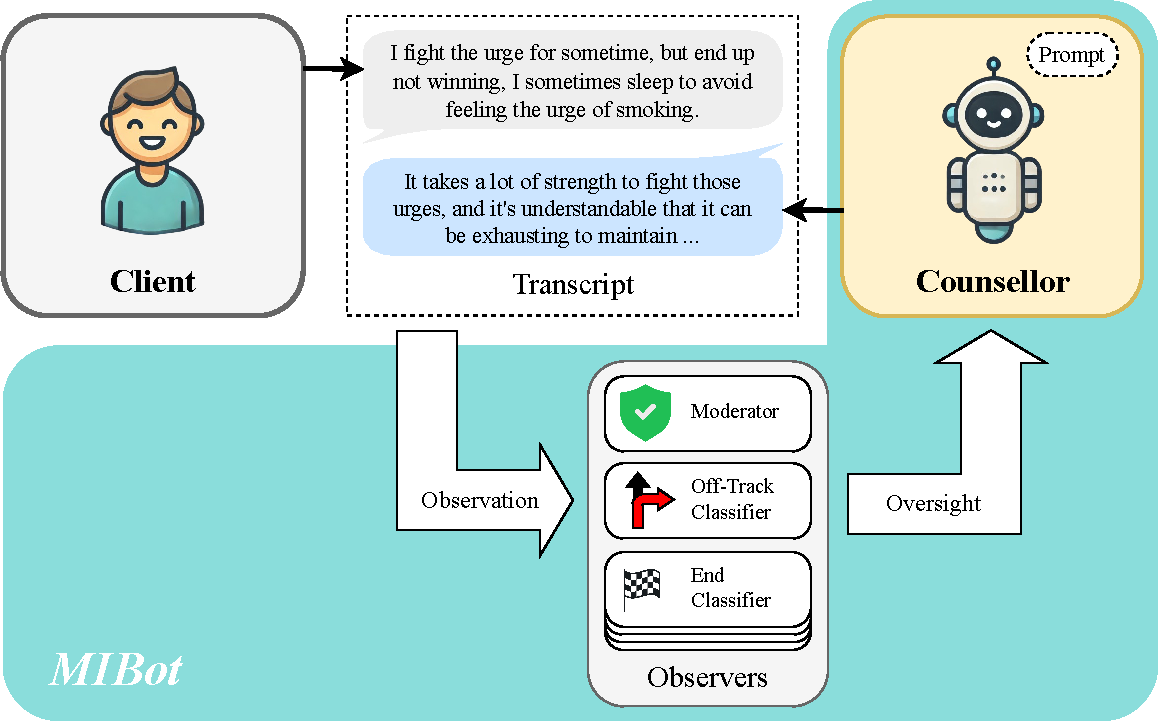
\includegraphics[width=0.8\linewidth]{fig/sysdiag.pdf}
    \caption{Overview of the \sysname system and observer agents.}
    \label{fig:system}
\end{figure*}